\documentclass[tikz,border=10pt]{standalone}
\usepackage{tikz}
\begin{document}
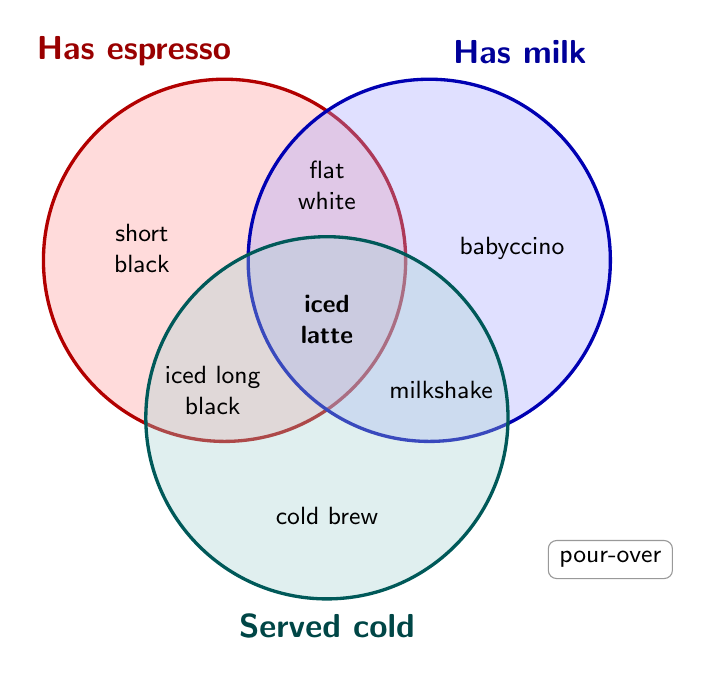
\begin{tikzpicture}[font=\sffamily]

  % Circle styles
  \tikzset{
    venncircle/.style={draw, line width=1.2pt, fill opacity=0.35, text opacity=1}
  }

  % Three overlapping circles
  \filldraw[venncircle, fill=red!40, draw=red!70!black]    (-1.3, 0.9) circle (2.3cm);
  \filldraw[venncircle, fill=blue!35, draw=blue!70!black]  ( 1.3, 0.9) circle (2.3cm);
  \filldraw[venncircle, fill=teal!35, draw=teal!70!black]  ( 0.0,-1.1) circle (2.3cm);

  % Circle labels (placed on the non-overlapping rim of each circle)
  \node[font=\sffamily\bfseries\large, text=red!60!black]  at (-2.45, 3.55) {Has espresso};
  \node[font=\sffamily\bfseries\large, text=blue!60!black] at ( 2.45, 3.55) {Has milk};
  \node[font=\sffamily\bfseries\large, text=teal!55!black] at ( 0.0, -3.75) {Served cold};

  % Drink labels

  % Espresso only: short black
  \node[align=center, font=\sffamily\small] at (-2.35, 1.05) {short\\black};

  % Milk only: babyccino
  \node[align=center, font=\sffamily\small] at (2.35, 1.05) {babyccino};

  % Cold only: cold brew
  \node[align=center, font=\sffamily\small] at (0.0, -2.35) {cold brew};

  % Espresso + Milk only (not cold): flat white
  \node[align=center, font=\sffamily\small] at (0.0, 1.85) {flat\\white};

  % Espresso + Cold only (no milk): iced long black
  \node[align=center, font=\sffamily\small] at (-1.45, -0.75) {iced long\\black};

  % Milk + Cold only (no espresso): milkshake
  \node[align=center, font=\sffamily\small] at (1.45, -0.75) {milkshake};

  % All three: iced latte
  \node[align=center, font=\sffamily\small\bfseries] at (0.0, 0.15) {iced\\latte};

  % None of the three: pour-over, outside all circles
  \node[align=center, font=\sffamily\small, draw=black!40, rounded corners=3pt,
        fill=white, inner sep=4pt] at (3.6, -2.9) {pour-over};

\end{tikzpicture}
\end{document}
